\documentclass[a4paper,12pt]{report}
\usepackage[utf8]{inputenc}
\usepackage[francais]{babel}
\usepackage{fancyhdr}
\usepackage{graphicx}
\usepackage{tikz}
\usetikzlibrary{calc}
\usepackage{listings}
\usepackage{xcolor}
\definecolor{grey}{rgb}{0.9,0.9,0.9}
\usepackage{titlesec}
\usepackage{verbatim}
\usepackage{listings}
\usepackage{textcomp}
\usepackage{hyperref}
\usepackage{longtable}
\usepackage{colortbl}
\usepackage{amssymb}

\definecolor{javakeyword}{rgb}{0,0,0.5}
\definecolor{javastring}{rgb}{0,0.5,0}
\definecolor{javacomment}{rgb}{0.5,0.5,0.5}
\lstdefinestyle{C++}{
   language=C++, basicstyle=\footnotesize,       % the size of the fonts that are used for the code
  numbers=left,                   % where to put the line-numbers
  numberstyle=\tiny\color{gray},  % the style that is used for the line-numbers
  stepnumber=1,                   % the step between two line-numbers. If it's 1, each line
                                  % will be numbered
  numbersep=5pt,                  % how far the line-numbers are from the code
  backgroundcolor=\color{white},  % choose the background color. You must add \usepackage{color}
  showspaces=false,               % show spaces adding particular underscores
  showstringspaces=false,         % underline spaces within strings
  showtabs=false,                 % show tabs within strings adding particular underscores
  frame=single,                   % adds a frame around the code
  rulecolor=\color{black},        % if not set, the frame-color may be changed on line-breaks within not-black text (e.g. commens (green here))
  tabsize=2,                      % sets default tabsize to 2 spaces
  captionpos=b,                   % sets the caption-position to bottom
  breaklines=true,                % sets automatic line breaking
  breakatwhitespace=false,        % sets if automatic breaks should only happen at whitespace
  title=\lstname,                 % show the filename of files included with \lstinputlisting;
   stringstyle=\color{javastring},
   keywordstyle=\color{javakeyword}\ttfamily\textbf,
   commentstyle=\color{javacomment}\ttfamily\textit
 }
\frenchbsetup{StandardLists=true}
\newcommand{\marge}{18mm}
\usepackage[left=\marge,right=\marge,top=\marge,bottom=\marge]{geometry}
\pagestyle{fancy}
\setlength{\headheight}{15pt}
\renewcommand{\headrulewidth}{1pt}
\linespread{1}
\setlength{\columnseprule}{0.2pt}
\title{TP3 VISA : stéréovision dense}
\author{NAIT ABDELAZIZ Yanis}


\begin{document}
\maketitle
\section*{Introduction}
Dans ce TP, nous allons utiliser la notion de similarité par SSD afin de déterminer si deux images représentent la même scène dans une configuraion canonique qui n'est rien d'autre qu'une translation de la caméra. Pour celà, nous allons utiliser tous les pixels des deux images et non que les coins comme dans le tp précédent en calculant la disparité des pixels qui est égale à la différence des abscisses de deux points homolgues. Nous allons travailler sur les deux images suivantes :
\begin{figure}[!ht]
	\center 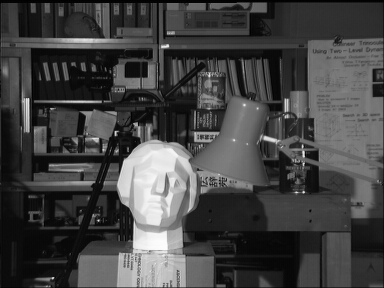
\includegraphics[scale=0.5]{./image/left.png}
			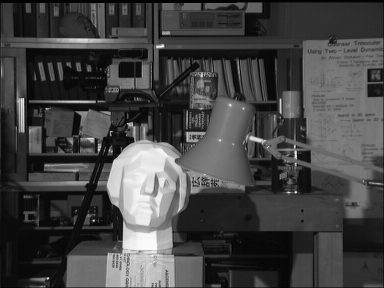
\includegraphics[scale=0.5]{./image/right.png}
\end{figure}

\section*{Similarité par SSD}
\subsection*{1-Images intermédiaires}
Dans cette partie de TP, nous allons dans un premier temps calculer la disparité entre les deux images en prenant comme référence l'image de gauche puis dans un deuxième temps l'image de droite. Le principe étant, pour chaque chaque pixel de procéder à un certain nombre de décalages soit vers la gauche soit vers la droite  dans mSSD la valeur de la somme des différences carrées des niveaux de gris des pixels contnus dans la fentre du décalage courant. Et si cette valeur est inféieure à la valeur de mMinSSD, cette dernière sera remplacée par la valeur de mSSD. Les valeurs de mMinSSD étant initialisées à un très grand nombre. L'utilisation des pointeurs dans le parcours des images rend plus facile la gestion des bords.\\
\noindent Le code ci-dessous permet de calculer la disparité pour tous les pixels de l'image de gauche avec les pixels de l'image de droite:
\begin{lstlisting}[style=C++]
Mat iviComputeLeftSSDCost(const Mat& mLeftGray,
                          const Mat& mRightGray,
                          int iShift,
                          int iWindowHalfSize) {
    Mat mLeftSSDCost(mLeftGray.size(), CV_64F);
    double value;
    for(int x=iWindowHalfSize;x<mLeftGray.size().height-iWindowHalfSize;x++){
        for(int y=iWindowHalfSize;y<mLeftGray.size().width-iWindowHalfSize;y++){
            value = 0.0;
            for(int i=-iWindowHalfSize;i<=iWindowHalfSize;i++){
                for(int j=-iWindowHalfSize;j<=iWindowHalfSize;j++){
                    value += pow(mLeftGray.at<uchar>(x+i,y+j)-mRightGray.at<uchar>(x+i,y+j-iShift),2);
                }
            }
            mLeftSSDCost.at<double>(x,y)=value;
        }
    }
    return mLeftSSDCost;
}
\end{lstlisting}
\noindent Ainsi la fonction minMaxLoc permet de récupérer les valeurs minimale et maximale contenues dans l'image précédemment calculée. La fonction normalize utilise ces deux valeurs pour normaliser toutes ces valeurs afin qu'elles soient comprises entre 0 et 255. L'affichage de ces valeurs normalisées nous permet donc d'obtenir l'image suivante :
\begin{figure}[!ht]
	\center
	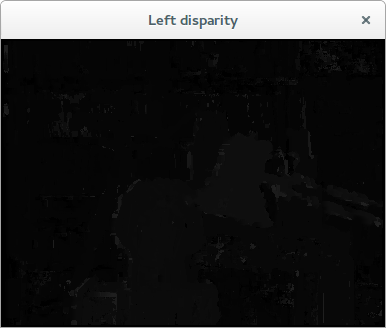
\includegraphics[scale=0.5]{./image/ld.png}
\end{figure}
\section*{Vérification gauche-droite}
Lorsqu'on prend l'image de droite comme référénce, la fonction est similaire à la fonction ci-dessus, seul le sens de décalage est inversé. L'affichage de l'image de disparité correspondante est la suivante :
\begin{figure}[!ht]
	\center 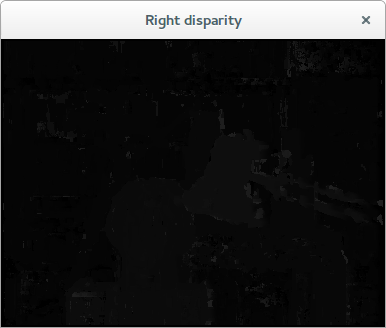
\includegraphics[scale=0.5]{./image/rd.png}
\end{figure} \\
Une fois que nous avons calculé les deux images de disparités correspondantes aux images gauche et droite, nous allons opérer à la procédure de vérification de correspondance decelles-ci qui consiste à parcourir les deux images de disparités et de vérifier si les valeurs de disparité deux pixels à la même position ont la même valeur. Si ces deux valeurs sont égale, alors on pourra considérer que ces pixels sont homolgues. Ainsi on reporte dans l'image masque un pixel noir et un pixel de la valeur de disparité dans l'image de disparité globale si les deux valeurs de disparités sont égales et un pixel noir dans le cas contraire. La fonction ci-dessous permet ainsi de décrire cette étape : 
\newpage
\begin{lstlisting}[style=C++]
Mat iviLeftRightConsistency(const Mat& mLeftDisparity,
                            const Mat& mRightDisparity,
                            Mat& mValidityMask){
    double dleft = 0.0;
    double disparityLeft = 0.0;
    double dright = 0.0;
    double disparityRight = 0.0;

    Mat mDisparity(mLeftDisparity.size(), CV_8U);

    for(int x=0;x<mLeftDisparity.rows;x++){
        for(int y=0;y<mLeftDisparity.cols;y++){

            dleft = (double)mLeftDisparity.at<uchar>(x,y);
            disparityLeft = (double)mRightDisparity.at<uchar>(x,y-dleft);

            dright = (double)mRightDisparity.at<uchar>(x,y);
            disparityRight = (double)mLeftDisparity.at<uchar>(x,y+dright);

            if(dleft!=disparityLeft || dright!=disparityRight){
                mValidityMask.at<uchar>(x,y)=255;
            }
            else{
                mDisparity.at<uchar>(x,y)=dleft;
                mValidityMask.at<uchar>(x,y)=0;
            }
        }
    }
    return mDisparity;
}
\end{lstlisting}
\noindent L'affichage des images de disparité globale et de masque nous permet d'avoir les résulats suivantes :
\begin{figure}[!ht]
	\center
	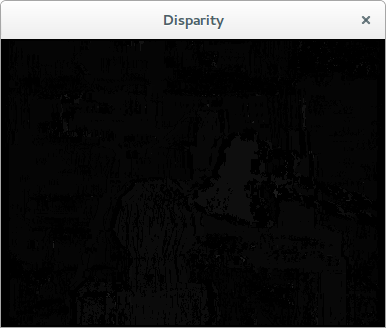
\includegraphics[scale=0.5]{./image/disparity.png}
	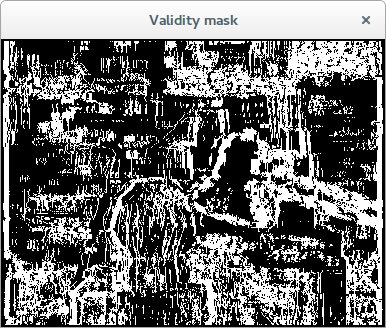
\includegraphics[scale=0.5]{./image/mask.png}
\end{figure}\\
\noindent Par analyse des images ci-dessus, on remarque que les points se trouvant à l'intérieur des contours des objets ont des homologues(pixels noir de l'image masque), et les points occultés étant représentés par des pixels blanc dans l'image masque. Dans l'image de disparité, tous les pixels noirs sont des pixels occultés.
\section*{Conclusion}
Dans ce TP, nous avons donc appris une nouvelle façon de vérifier la cohérence de deux images en configuration canonique notamment en calculant la disparité des pixels de chaque image en retenant la valeur minimale de tous les décalages effectués, ainsi à partir de ces images de disparités on peut facilement déterminer les points homolgues. Cependant, on peut remarquer que cette procédure n'est pas très efficace en terme de temps de calcul.
\end{document}